\documentclass[a4paper, 12pt]{article}
\usepackage[T2A]{fontenc}
\usepackage[utf8]{inputenc}
\usepackage[english,russian]{babel}
\usepackage{amsmath, amsfonts, amssymb, amsthm, mathtools, misccorr, indentfirst, multirow}
\usepackage{wrapfig}
\usepackage{graphicx}
\usepackage{subfig}
\usepackage{adjustbox}
\usepackage{pgfplots}

\usepackage{siunitx}
\usepackage{circuitikz}
\usepackage{geometry}
\geometry{top=20mm}
\geometry{bottom=20mm}
\geometry{left=20mm}
\geometry{right=20mm}
\newcommand{\angstrom}{\textup{\AA}}
\begin{document}
\begin{titlepage}
    \newpage
    \begin{center}
     Министерство науки и высшего образования Российской федерации \\ ФЕДЕРАЛЬНОЕ ГОСУДАРСТВЕННОЕ АВТОНОМНОЕ \\ ОБРАЗОВАТЕЛЬНОЕ УЧРЕЖДЕНИЕ ВЫСШЕГО ОБРАЗОВАНИЯ \\ «МОСКОВСКИЙ ФИЗИКО-ТЕХНИЧЕСКИЙ ИНСТИТУТ \\ (НАЦИОНАЛЬНЫЙ ИССЛЕДОВАТЕЛЬСКИЙ УНИВЕРСИТЕТ)» \\ (МФТИ, Физтех)
    \end{center}
    
    \vspace{15em}
    
    \begin{center}
    КАФЕДРА ТВЕРДОТЕЛЬНОЙ ЭЛЕКТРОНИКИ \\
    \vspace{1em}
    ОТЧЕТ\\
    ПО ЛАБОРАТОРНОЙ РАБОТЕ \\
    \vspace{1em}
    ОПРЕДЕЛЕНИЕ ШИРИНЫ ЗАПРЕЩЕННОЙ ЗОНЫ ПОЛУПРОВОДНИКОВ ПО СПЕКТРАЛЬНОЙ ЗАВИСИМОСТИ СОБСТВЕННОЙ ФОТОПРОВОДИМОСТИ
    \end{center}

    \vspace{10em}
    \begin{flushleft}
        Работу выполнили \hspace{17em} \underline{\hspace{3cm}}
        И.Д. Бессонов \\
         \hspace{26em} \underline{\hspace{3cm}} Е.С. Иванова \\
          \hspace{26em} \underline{\hspace{2.6cm}} Е.О. Коробкина\\
          \hspace{26em} \underline{\hspace{3cm}} А.А. Макоткин\\
        \hspace{26em}
        \raisebox{-\baselineskip}{\shortstack{\underline{\hspace{3cm}}\\(подпись, дата)}}     
        И.С. Потапова
    \end{flushleft}

    \vspace{1em}

    \begin{flushleft}
        Работу принял, оценка
        \hspace{15em}
        \raisebox{-\baselineskip}{\shortstack{\underline{\hspace{5cm}}\\(подпись, дата, оценка)}}
    \end{flushleft}

    \vspace{5em}
    
    \begin{center}
        Долгопрудный, 2025
    \end{center}
\end{titlepage}

\newpage
\tableofcontents

\newpage
\section{Аннотация}
\textbf{Цель работы:} ознакомиться с основами теории собственной фотопроводимости полупроводников, определить ширину запрещённой зоны кремния по спектральной зависимости собственной фотопроводимости и найти скорость поверхностной рекомбинации.

    
   

\section{Теоретическая часть}
При воздействии на полупроводник излучения с энергией кванта $h\nu$, превышающей ширину запрещённой зоны $E_g$ в зоне проводимости, и соотвественно в валентной зоне возникают неравновесные электроны и дырки. Их появление связано с переходами электронов из валентной зоны проводимости. В результате увеличивается проводимость кристалла. Это явление называется собственной фотопроводимостью.

В непрямозонных полупроводниках типа германия и кремния минимум зоны проводимости и максимум валентной зоны расположены в различных точках зоны Бриллюэна. В этом случае оптический переход электрона из вершины валентной зоны в минимум зоны проводимости возможен лишь при участии третьей частицы – фонона. В соответствии с законом сохранения импульса квазиимпульс такого фонона $q_{\text{ф}}\approx\hbar k_{\text{Б}}$, а энергия $\hbar\omega$ должна удовлетворять закону сохранения энергии:
    \begin{equation}
        h\nu = E_g\pm \hbar\omega_q+\hbar^2(k_n-k_c)^2/2m_n+\hbar^2k_p^2/2m_p
    \end{equation}
    где $k_n$ и $k_p$ -- начальные волновые числа электрона и дырки, а $k_c$ -- конечное волновое число электрона.

Таким образом, край основной полосы поглощения в полупроводниках типа кремния и германия определяется непрямыми оптическими переходами, сопровождающимися поглощением и испусканием фононов. При этом для разрешённых переходов, которые доминируют в полупроводниках такого типа, коэффициент поглощения:

    \begin{equation}
        K=C\left[\frac{(h\nu-E_g+\hbar\omega_q)^2}{\exp{\frac{\hbar\omega_q}{kT}}-1}+\frac{(h\nu-E_g-\hbar\omega_q)^2}{1-\exp{-\frac{\hbar\omega_q}{kT}}}\right]
    \end{equation}
При больших энергиях квантов $h\nu>(E_g+\hbar\omega_q)$ начинают преобладать переходы с эмиссией фононов и зависимость $K^{1/2}$ от $h\nu$ должна аппроксимироваться прямой, пересекающей ось энергии в точке $h\nu_1=E_g+\hbar\omega_q$.

При рассмотрении случая сильного поглощения излечения в образце (оптически толстый образец), то есть при $d/K<<1$, где $d$ -- толщина образца, скорость генерации электронно-дырочных пар экспоненциально уменьшается от поверхности вглубь образца:
    \begin{equation}
        g(x)\approx K(1-R)N_0\exp{-Kx}
    \end{equation}
    где $R$ -- коэффициент отражения света, а $N_0$ -- поток квантов на единицу поверхности.

Неоднородная германия электронов и дырок в направлении освещения приводит к появлению диффузионно-дрейфовых потоков носителей заряда: быстро диффундирующие носители (электроны) опережают медленные (дырки), что приводит к возникновению электрического поля, ускоряющего медленные носители и замедляющего быстрые и к появлению дрейфовых составляющих потоков. При этом изменение проводимости $\Delta\Sigma$ существенным образом зависит от граничных условий на поверхности образца:
    \begin{equation}
        \Delta\Sigma\sim N_0\left(1+\frac{S}{D}\frac{1}{K}\right)
    \end{equation}
    где $S$ -- скорость поверхностной рекомбинации, $D$ -- коэффициент амбиполярной диффузии.





\section{Экспериментальная часть}
\subsection{Экспериментальная установка}
    Для изменения фотоответа полупроводника $\Delta\Sigma$ образец включается последовательно с нагрузочным сопротивлением и источником постоянного напряжения. При освещении проводимость образца возрастает, происходит перераспределение напряжение между образцом и нагрузкой. В результате падение напряжения $U$ на образце при малом относительном увеличении проводимости уменьшается на величину
    \begin{equation}
        \Delta U=\varepsilon\frac{R_H\cdot R_0^2}{(R_H+R_0)^2}\Delta\Sigma
        \label{eq:deltaU}
    \end{equation}
    где $\varepsilon$ -- постоянное напряжение, $R_H$ и $R_0$ -- сопротивление нагрузки и образца, $\Sigma$ -- проводимость.

    Для повышения чувствительности измерения обычно проводят при периодическом прерывании светового потока. При этом соотношение (\ref{eq:deltaU}) характеризует амплитуду отрицательных импульсов напряжения на концах образца. Для исследования интересующих нас зависимостей $\Delta\Sigma/N_0$ от энергии кванта $h\nu$ наряду с $\Delta U$ необходимо знать спектральное распределение интенсивности источника излучения $N_0(h\nu)$.
    \begin{figure}[!htb]
        \centering
        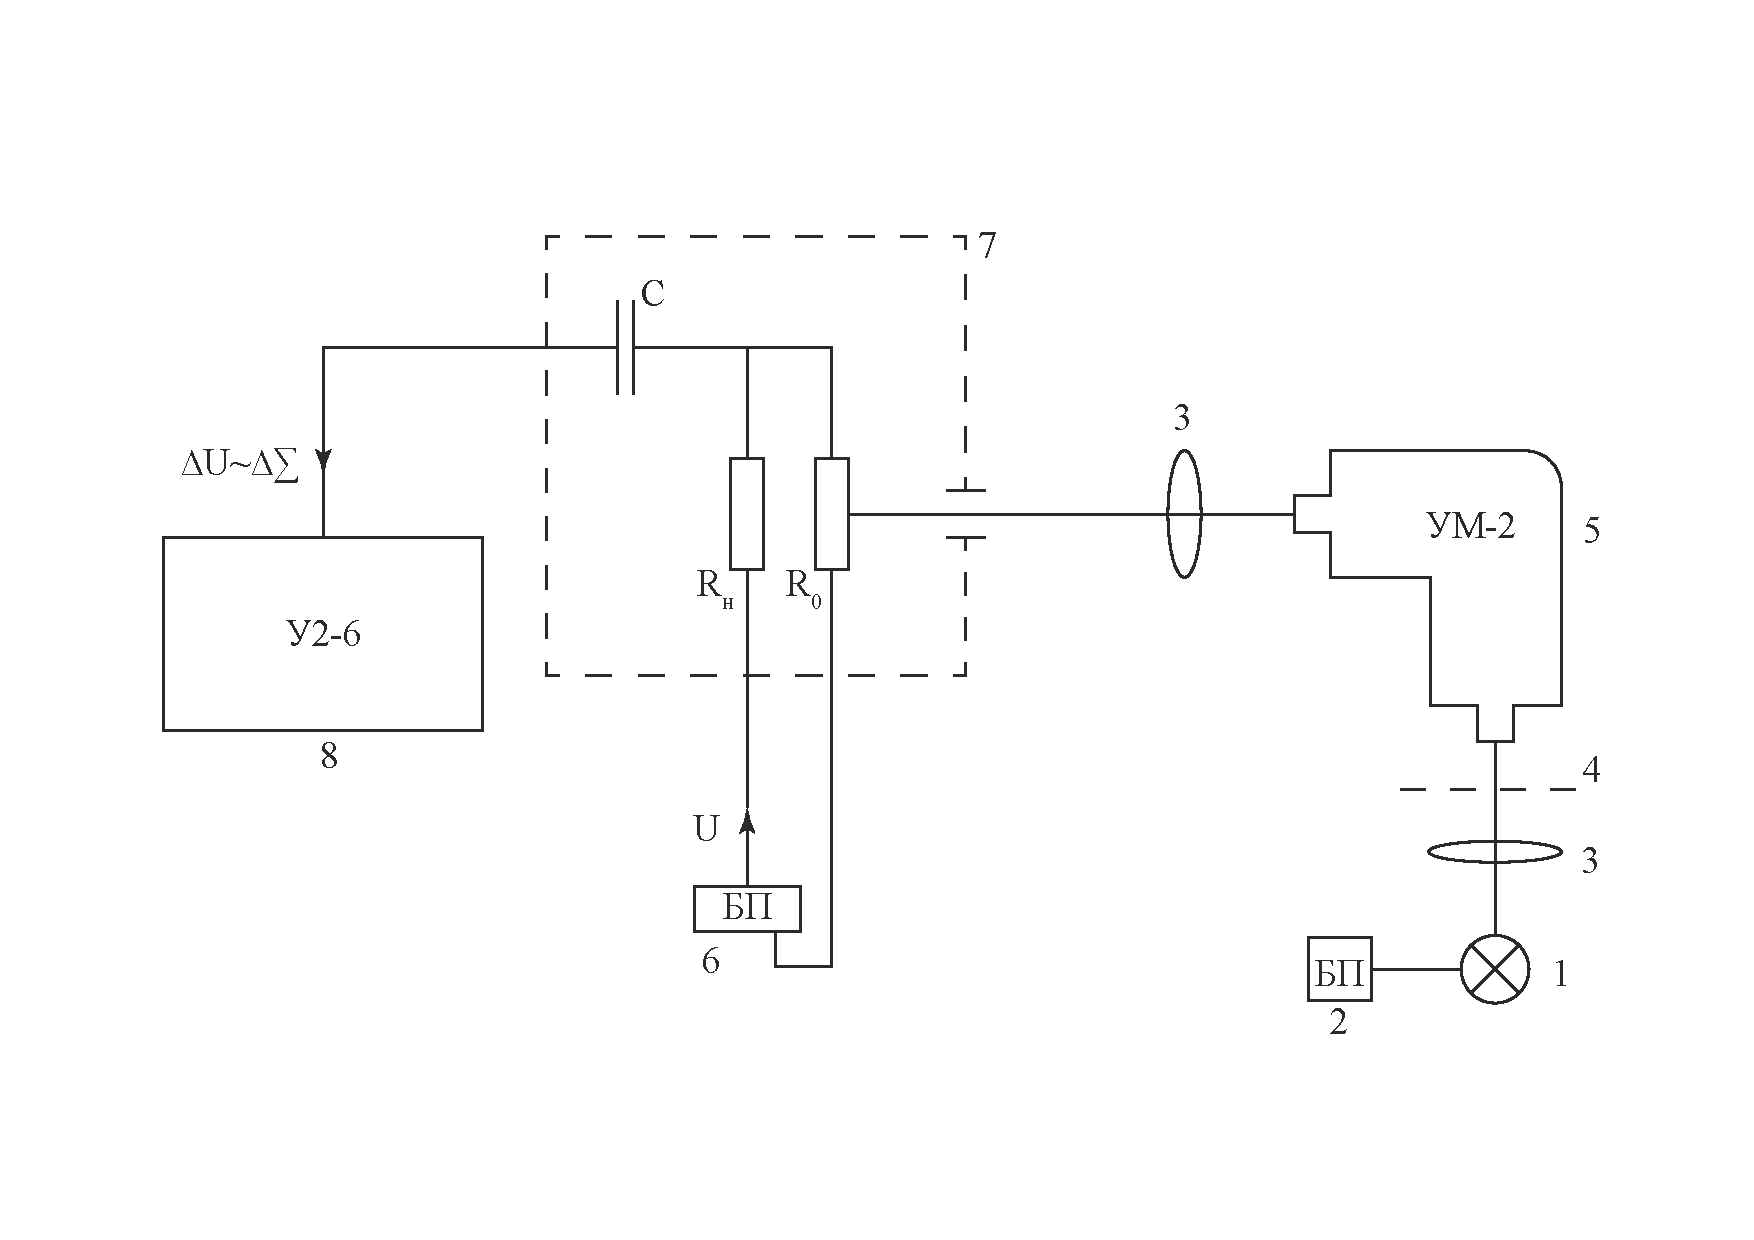
\includegraphics[width=\textwidth]{img/exp_scheme.pdf}
        \caption{Схема экспериментальной установки. 1 -- осветитель, 2 -- блок питания осветителя, 3 -- линзы, 4 -- механический модулятор излучения, 5 -- монохроматор, 6 -- блок питания образца, 7 -- схема включения образца, 8 -- усилитель}
    \end{figure}
\section{Ход работы}
 
    Включаем лампу накаливания и фокусируем излучение монохроматора на образец Si. Подаём постоянное смещение $U$ на образец от источника напряжения. Вращая барабан длин волн, снимаем зависимость сигнала фотопроводимости $\Delta U$ от длины волны излучения. С помощью графика спектрального распределения интенсивности лампы составляем таблицу $(\Delta Uh\nu)/I_0$ от делений барабана. С помощью градуировочной кривой переводим деления барабана в энергии кванта $h\nu$. Получаем зависимость $(\Delta Uh\nu)/I_0(h\nu)$, после чего строим зависимость $\sqrt{(\Delta Uh\nu)/I_0}(h\nu)$.
    \begin{figure}[h!]
\begin{center}
\begin{minipage}[h!]{0.495\linewidth}
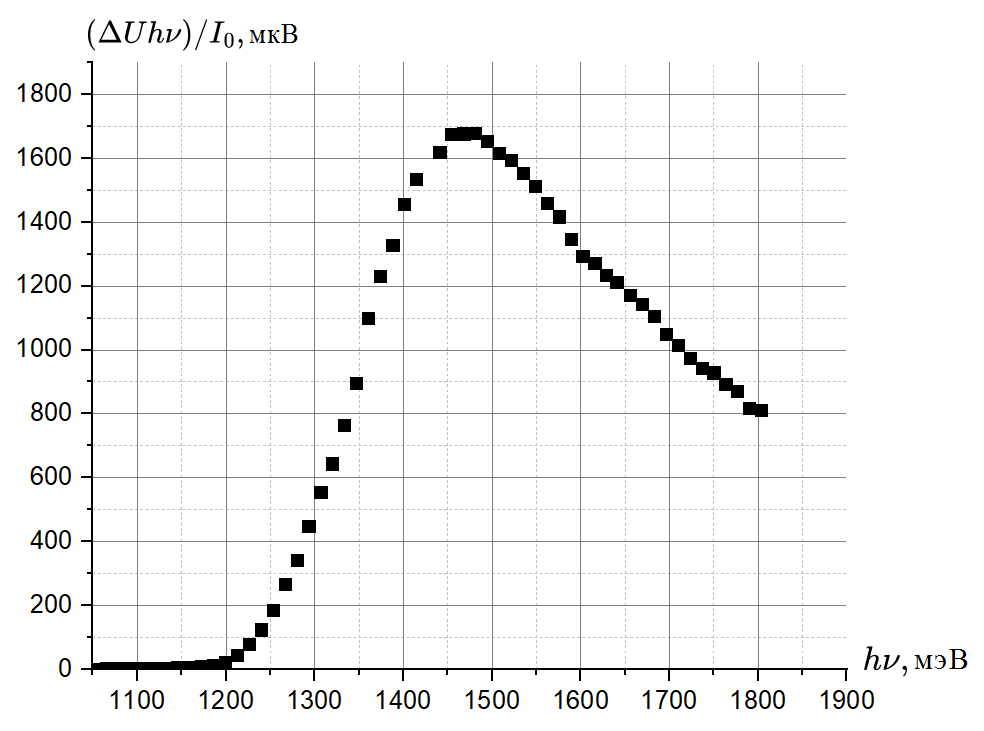
\includegraphics[width=1\linewidth]{img/l1.png}
\label{ris:experimoriginal} %% метка рисунка для ссылки на него
\end{minipage}
\hfill 
\begin{minipage}[h!]{0.495\linewidth}
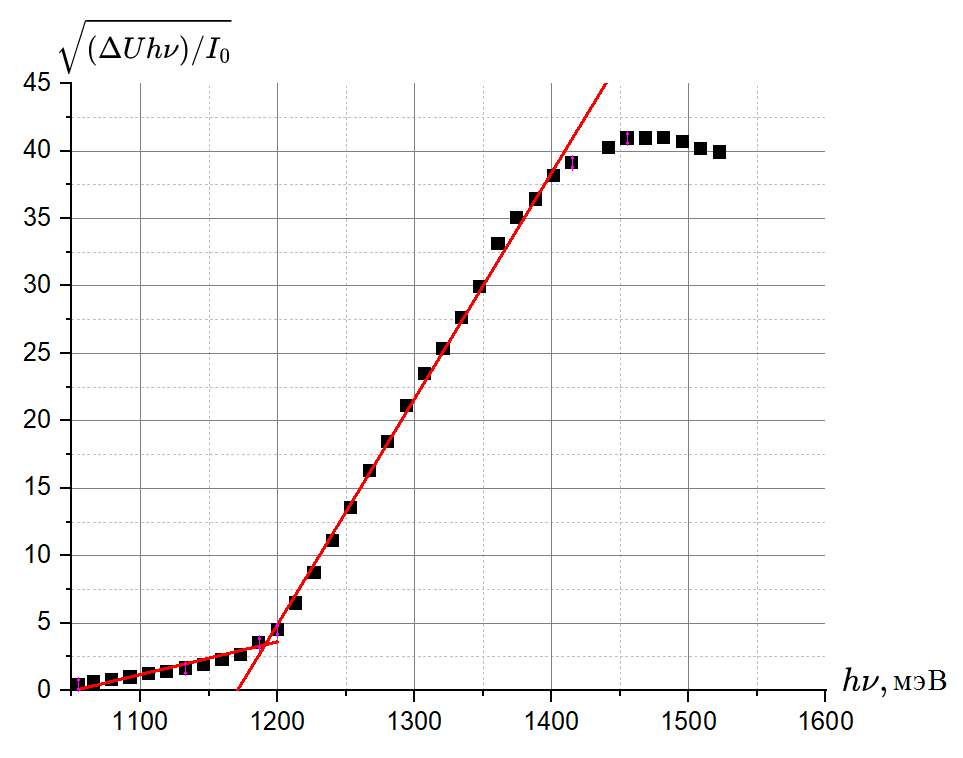
\includegraphics[width=1\linewidth]{img/l2.png}

\label{ris:experimcoded}

\end{minipage}
\caption{\centering{График зависимостей $(\Delta Uh\nu)/I_0(h\nu)$ и $\sqrt{(\Delta Uh\nu)/I_0}(h\nu)$ через пластинку кремния.}}
\end{center}
\end{figure}

 \begin{figure}[h!]
\begin{center}
\begin{minipage}[h!]{0.495\linewidth}
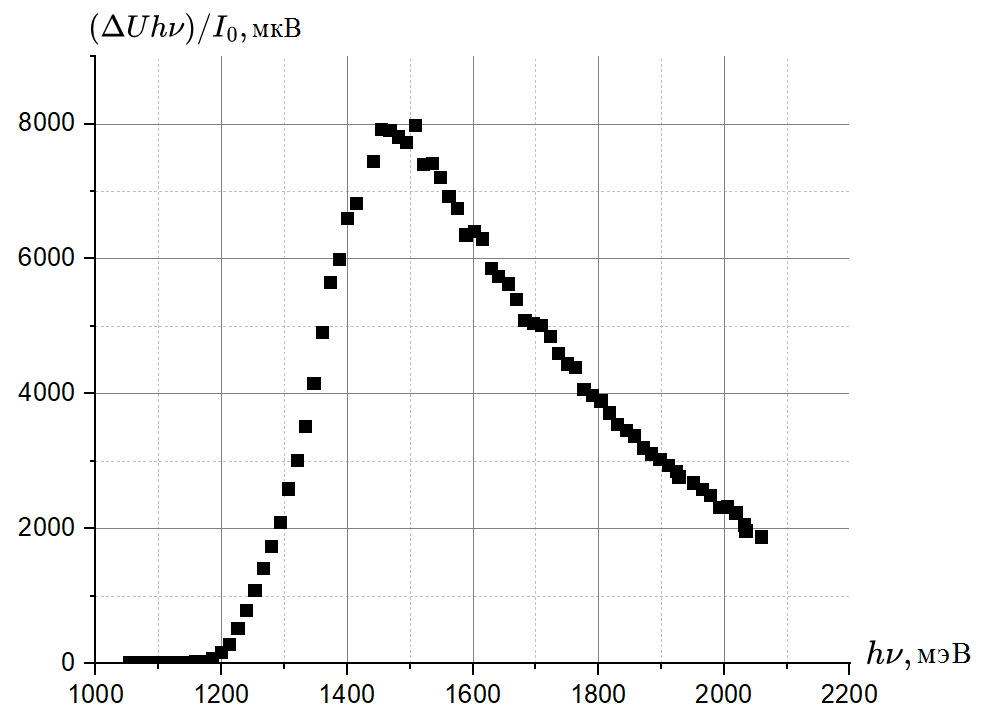
\includegraphics[width=1\linewidth]{img/l7.png}
\label{ris:experimoriginal} %% метка рисунка для ссылки на него
\end{minipage}
\hfill 
\begin{minipage}[h!]{0.495\linewidth}
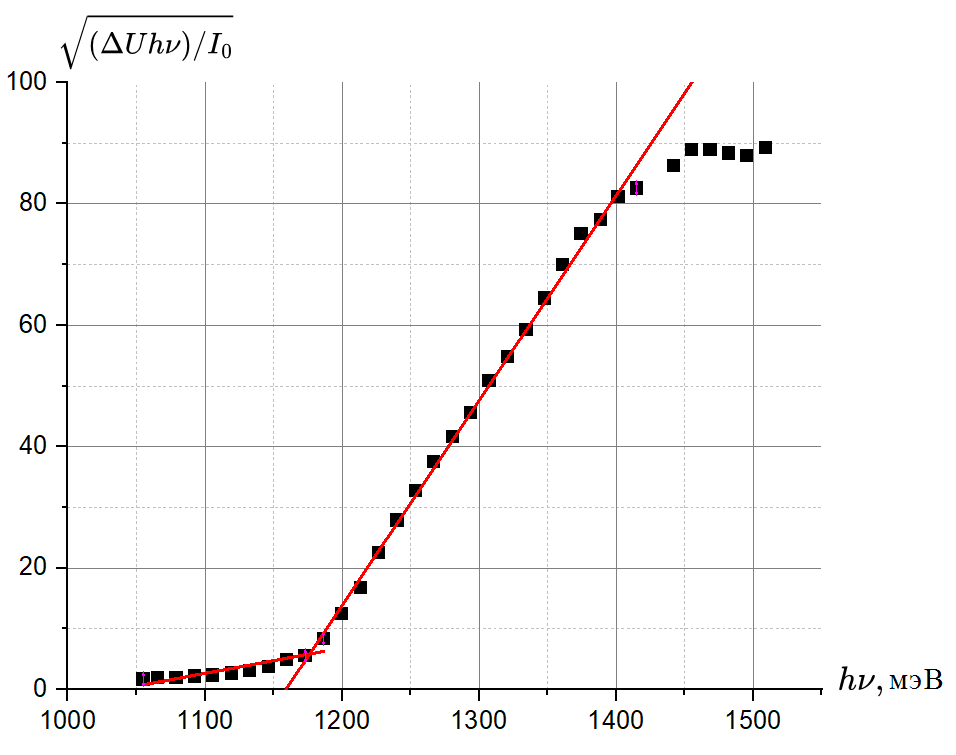
\includegraphics[width=1\linewidth]{img/l8.png}

\label{ris:experimcoded}

\end{minipage}
\caption{График зависимостей $(\Delta Uh\nu)/I_0(h\nu)$ и $\sqrt{(\Delta Uh\nu)/I_0}(h\nu)$  на кремнии без фильтра.}
\end{center}
\end{figure}



\begin{figure}[h!]
\begin{center}
\begin{minipage}[h!]{0.495\linewidth}
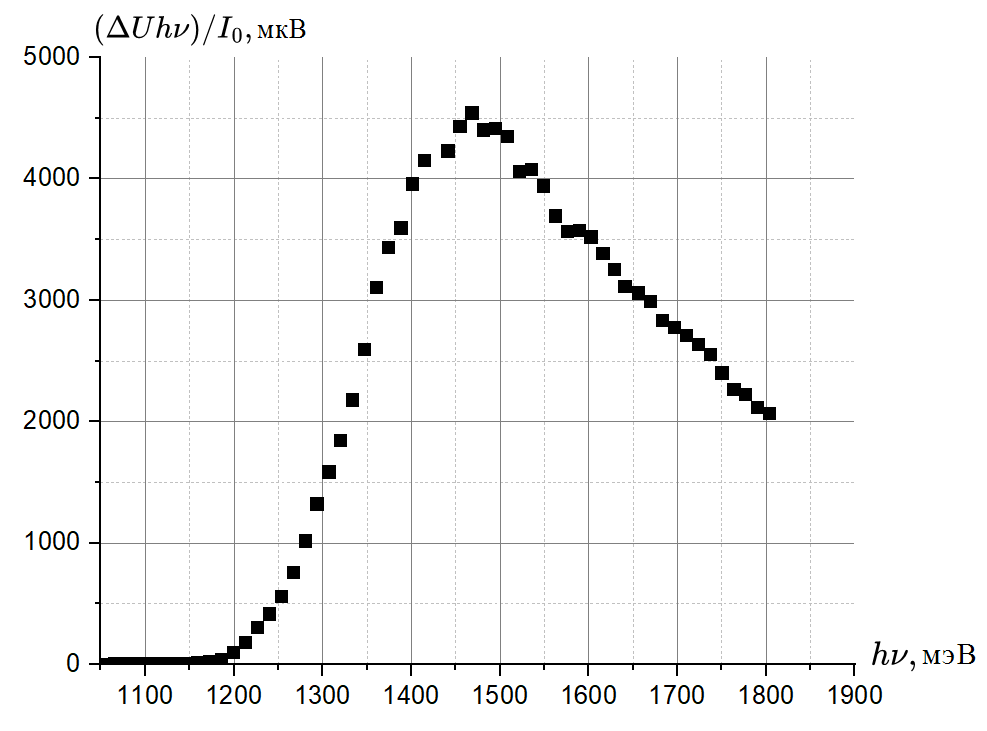
\includegraphics[width=1\linewidth]{img/l4.png}
\label{ris:experimoriginal} %% метка рисунка для ссылки на него
\end{minipage}
\hfill 
\begin{minipage}[h!]{0.495\linewidth}
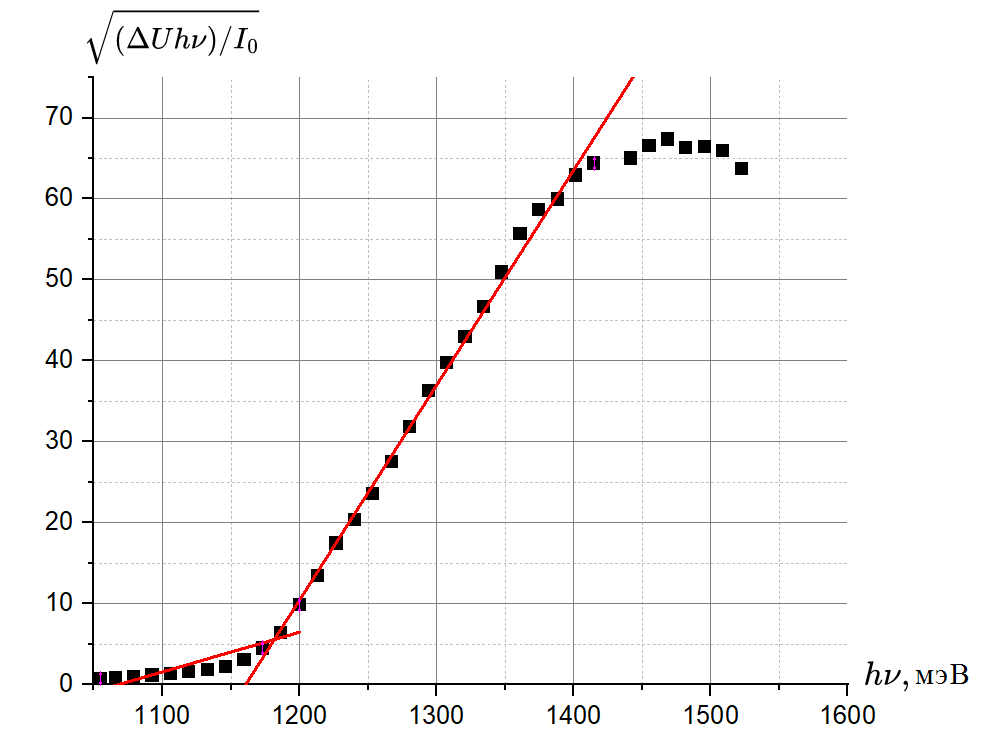
\includegraphics[width=1\linewidth]{img/l5.png}

\label{ris:experimcoded}

\end{minipage}
\caption{\centering{График зависимостей $(\Delta Uh\nu)/I_0(h\nu)$ и $\sqrt{(\Delta Uh\nu)/I_0}(h\nu)$ через пластинку кремния (наш).}}
\end{center}
\end{figure}
  
   

Аппроксимируя линейный участок графика зависимости $\sqrt{(\Delta Uh\nu)/I_0}(h\nu)$ до оси энергии, получаем величину $(E_g+\hbar\omega_{\text{ф}})$ как точку пересечения прямой с осью. Учитывая энергию фонона $\hbar\omega_{\text{ф}}=50$ мэВ, находим ширину запрещённой зоны кремния $E_g\approx1100$ мэВ.
\newpage
\begin{figure}[h!]
\begin{center}
\begin{minipage}[h!]{0.495\linewidth}
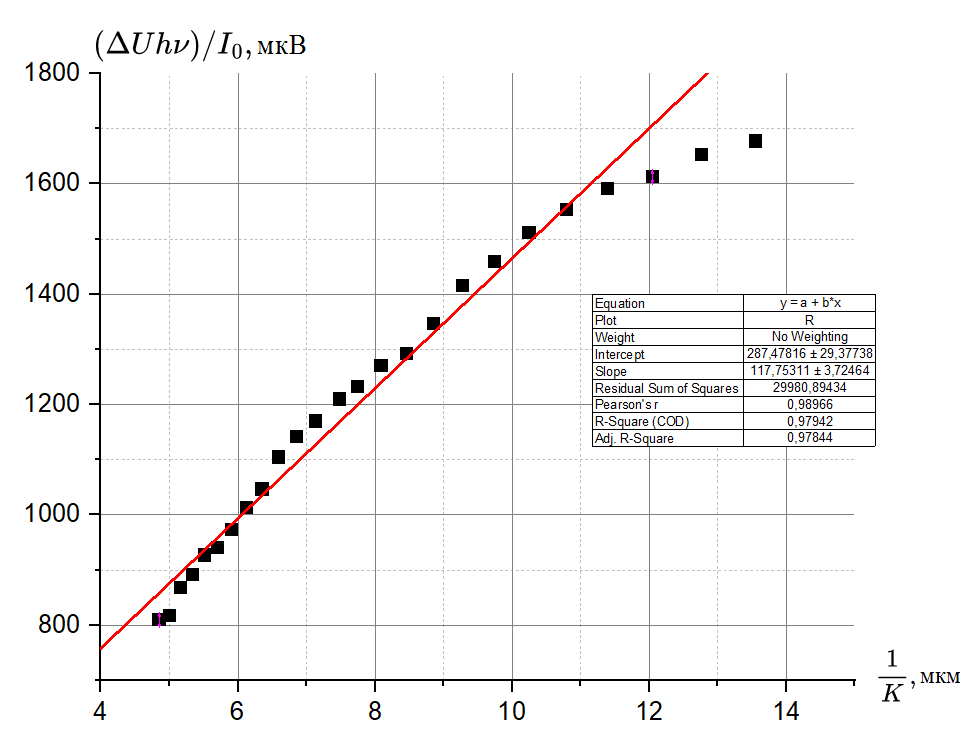
\includegraphics[width=1\linewidth]{img/l3.png}
\label{ris:experimoriginal} %% метка рисунка для ссылки на него
\end{minipage}
\hfill 
\begin{minipage}[h!]{0.495\linewidth}
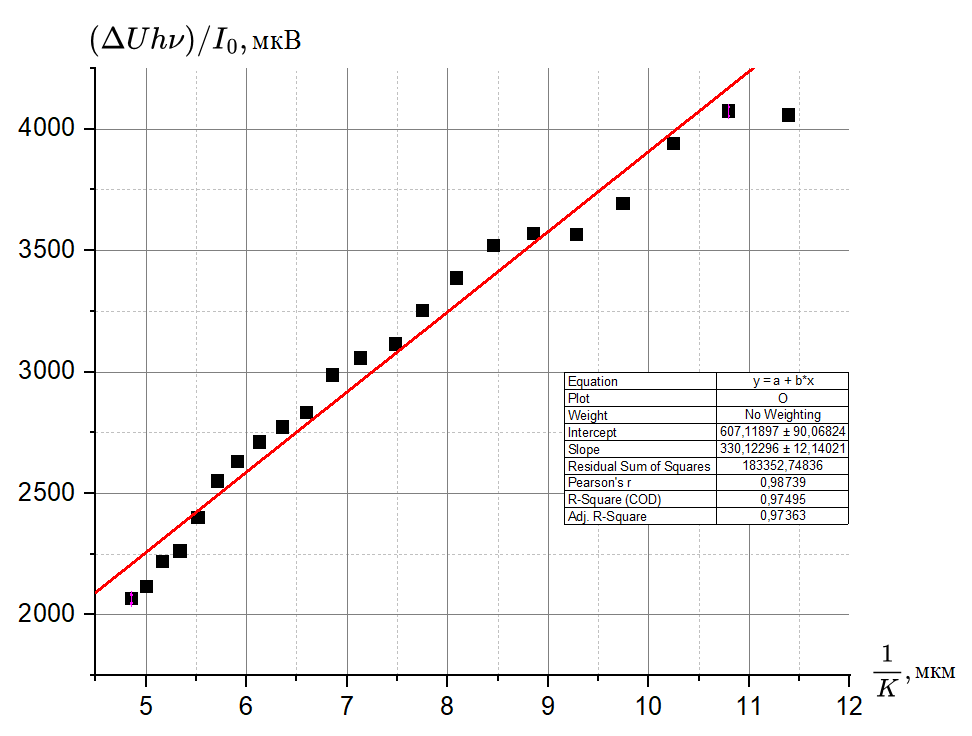
\includegraphics[width=1\linewidth]{img/l6.png}

\label{ris:experimcoded}

\end{minipage}
\hfill 
\begin{minipage}[h!]{0.495\linewidth}
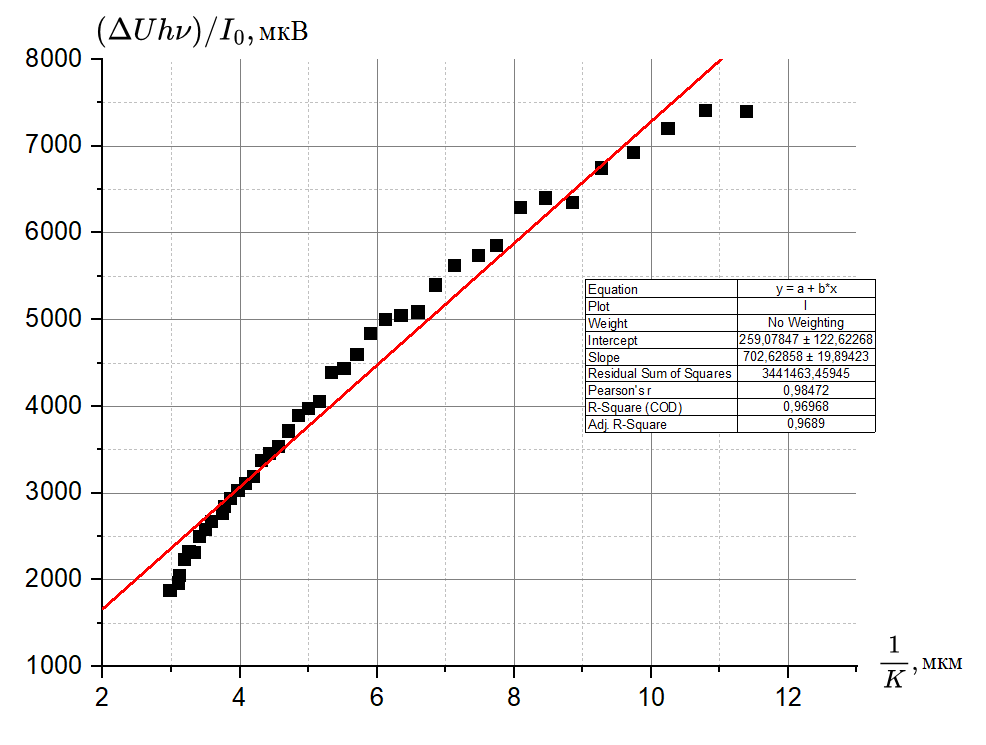
\includegraphics[width=1\linewidth]{img/l9.png}

\label{ris:experimcoded}

\end{minipage}

\caption{\centering{График зависимости $(\Delta Uh\nu)/I_0(\frac{1}{K})$ при $Kd \gg 1$.}}
\end{center}
\end{figure}


Строим зависимость $(\Delta Uh\nu)/I_0(\frac{1}{K})$. Аппроксимируя график, получаем скорости поверхностной рекомбинации кремния: $s_1=1,17\cdot10^{4} \; \frac{\text{см}}{\text{с}}; \; s_2=3,3\cdot10^{4} \; \frac{\text{см}}{\text{с}}; \; s_3=7\cdot10^{4} \; \frac{\text{см}}{\text{с}}$.


\section{Выводы}
\begin{enumerate}
\item Изучили принципы собственной фотопроводимости в полупроводниках.
\item Экспериментально определили ширину запрещенной зоны кремния: $E_g\approx1100$ мэВ.
\item Определили скорости поверхностной рекомбинации кремния для трех измерений: $s_1=1,17\cdot10^{4} \; \frac{\text{см}}{\text{с}}; \; s_2=3,3\cdot10^{4} \; \frac{\text{см}}{\text{с}}; \; s_3=7\cdot10^{4} \; \frac{\text{см}}{\text{с}}$.
\end{enumerate}

\section{Ответы на вопросы к лабораторной работе №3}
\begin{enumerate}
\itemЧто такое скорость оптической генерации? Её размерность?
$$ g(x)= \frac{dn}{dt}=[\frac{1}{\text{м}^3\text{с}}] \; - \; \text{скорость создания пар электрон+дырка в данном объеме вещества}.$$   
    
\itemРазъяснить понятие «оптически тонкий образец».

Понятие «оптически тонкий образец» означает, что свет, проходя через такой образец, практически не изменяет свою интенсивность, то есть слабо поглощается. Пусть $k \; - \;$коэффициент поглощения в веществе, из которого сделан образец, $d \; - \;$его толщина, тогда условие оптически тонкого образца записывается в виде: $kd \ll 1$.


\itemПолучить выражение для скорости оптической генерации в случае, когда образец можно считать оптически тонким.

Считаем, что потери идут только на возбуждение электрона, тогда:
$$g(x)=\frac{j_{\text{ф}}kSdx}{Sdx}e^{-kx} + j_{\text{ф}}ke^{-k(d-x)}e^{-kd}R + j_{\text{ф}}ke^{-kx}e^{-2kd}R^2 + ...= j_{\text{ф}}k (e^{-kx}+Re^{-k(d-x)}) \sum \limits_{n=0}^{\infty} (Re^{-kd})^{2n}$$

где первое слагаемое - это отражение от прямой волны, второе - от отразившейся один раз волны, третье - от отразившейся два раза волны и так далее. Причем R - коэффициент отражения, $e^{-kd}$ - ослабление интенсивности света при прохождении через образец, $j_{\text{ф}}$ - число фотонов в прогонке. Применяя формулу для суммы геометрической прогрессии, получаем:

$$g(x)= \frac{j_{\text{ф}}k}{1-(Re^{-kd})^2}(e^{-kx}+Re^{-k(d-x)})$$

Считаем, что $j_{\text{ф}}=\frac{I_0(1-R)}{h\nu}$, где $I_0$ - интенсивность падающего света, а $h\nu$ - энергия одного фотона. Условие оптически тонкого образца: $kd \ll 1$, тогда $e^{-kd}=1-kd$. В итоге:
$$g(x)=\frac{I_0k(1-R)}{h\nu(1-R^2(1-kd)^2)}(1-R)=\frac{I_0k(1+R)}{h\nu(1-R^2)}(1-R)=\frac{I_0k}{h\nu}.$$

\itemКак зависит фотопроводимость от коэффициента поглощения при энергиях света, когда образец можно считать оптически тонким? Оптически толстым?\par
В оптически толстом образце $Kd>>$1 и
\begin{equation}
    g(x) = kN_0(1-R)e^{-kx}
\end{equation}
Тогда система уравнений непрерывности примет вид:
\begin{equation}
    kN_0(1-R)e^{-kx}=\frac{\Delta n}{\tau_n}=\frac{\Delta p}{\tau_p}
\end{equation}
Экспонента убывает сильнее, тогда решив уравнения, можно сказать, что изменение проводимости образца $\Delta \sum \approx \frac{1}{K}$\par
Для оптически тонкого образца $\Delta \sum \approx K$\par
\itemРассчитать коэффициент пропорциональности между энергией кванта света в эВ и соответствующей длиной волны в мкм.
\begin{equation}
    E = h\nu = \frac{hc}{\lambda}
\end{equation}
Значение $hc$ и есть коэффициент пропорциональности между энергией и длиной волны.
\begin{equation}
    hc = 1.05 \cdot 10^{-24}\cdot 2\pi \cdot 2\cdot 10^{10}= 19.8 \cdot 10^{-17} \text{ эрг*см} = 19.8\cdot 10^{-17} \cdot 6.24\cdot 10^{11}\text{ эВ*см}
\end{equation}
Окончательно,
\begin{equation}
    hc =12.4 \cdot 10^{-5} \cdot 10^{4} \text{ эВ*мкм}=1.24 \text{ эВ*мкм}
\end{equation}

\itemШирина зоны прямозонного полупроводника 0,8 эВ. Чтобы определить длину волны, при которой можно наблюдать собственную фотопроводимость в прямозонном полупроводнике, воспользуемся соотношением между шириной запрещённой зоны \(E_g\) и длиной волны \(\lambda\) света:

\[\lambda = \frac{hc}{E_g}.\]

Подставив значения, найдем длину волны, при которой можно наблюдать собственную фотопроводимость:

\[\lambda = \frac{(4.135667696 \times 10^{-15} \, \text{эВ·с}) \cdot (3 \times 10^8 \, \text{м/с})}{0.8 \, \text{эВ}} \approx 1.55 \, \text{мкм} .\]

\itemТемновое сопротивление фоторезистора составляет 40 кОм. Для получения максимального сигнала на фоторезисторе необходимо согласовать нагрузочное сопротивление с темновым сопротивлением фоторезистора, что следует из \textbf{теоремы о максимальной мощности: }максимальная мощность передаётся в нагрузку, когда сопротивление нагрузки равно внутреннему сопротивлению источника.

Мощность, выделяемая на нагрузке, определяется формулой:
\[P = I^2 R_{\text{нагр}},\]
где \( I \) — ток в цепи, который зависит от напряжения источника и общего сопротивления (фоторезистор + нагрузка):
\[I = \frac{U}{R_{\text{темн}} + R_{\text{нагр}}},\]

\begin{center}
\begin{circuitikz}[european resistors]

    % Источник напряжения
    \draw (0,0) to[battery1, l=$V$] (0,3);

    % Фоторезистор
    \draw (0,3) to[photoresistor, l=$R_{\text{фото}}$, *-*] (3,3);

    % Нагрузочное сопротивление
    \draw (3,3) to[resistor, l=$R_{\text{нагр}}$, *-*] (3,0);

    % Замыкание цепи
    \draw (3,0) -- (0,0);
\end{circuitikz}
\end{center}

Таким образом, при \( R_{\text{нагр}} = R_{\text{темн}} = 40 \, \text{кОм} \) достигается баланс между током и напряжением, что обеспечивает максимальный сигнал (максимум мощности).
\itemЧтобы найти на какое расстояние успеют продиффудировать избыточные электроны в Si, если время жизни носителей составляет \( \tau = 10^{-4} \, \text{с}\), воспользуемся уравнением диффузии:

\[L = \sqrt{D \tau},\]
где \( L \) — диффузионное расстояние и \( D \) — коэффициент диффузии электронов,

Для кремния при комнатной температуре (300 K) коэффициент диффузии электронов:
   \[D \approx 36 \, \text{см}^2/\text{с}, \]
   поскольку \[D = \mu V_T,\]
   где \( \mu = 1400 \, \text{см}^2/\text{В·с} \) — подвижность электронов, а \( V_T = \frac{kT}{q} \approx 0.0259 \, \text{В} \) — тепловое напряжение.
   Подставляем значения в формулу:
   \[L = \sqrt{D \tau} = \sqrt{(36 \times 10^{-4} \, \text{м}^2/\text{с}) \cdot (10^{-4} \, \text{с})} = 600 \, \text{мкм}.\]
Если температура или другие параметры отличаются от стандартных, коэффициент диффузии \( D \) будет другим, и результат изменится.
 

\itemНа Рис. 4 показаны спектральные зависимости фотопроводимости CdS  и CdSe. Пунктирные и сплошные линии соответствуют разным температурам.

    \begin{figure}[!h]
        \centering
        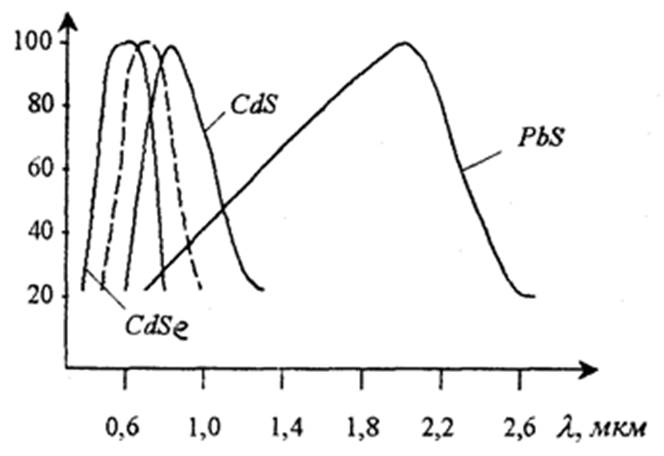
\includegraphics[scale=0.7]{img/9.png}
        \caption{}
    \end{figure}
    Для CdS и CdSe ширина запрещённой зоны определяет длину волны, при которой наблюдается максимальная фотопроводимость. Таким образом, при низких температурах пик фотопроводимости соответствует \(E_g\), а при высоких температурах пик сглаживается из-за тепловой генерации носителей.
    
Сплошные линии на графике соответствуют низким температурам, где фотопроводимость более выражена и определяется в основном поглощением света. Пунктирные линии соответствуют высоким температурам, где тепловые эффекты сглаживают спектральную зависимость. Это связано с физикой фотопроводимости и влиянием температуры на полупроводниковые материалы.
\item Нарисуйте качественно зависимость сигнала фотопроводимости кремниевого фоторезистора от энергии кванта. Энергия фонона $\approx$ 50 мэВ.

Кремний (Si) является  непрямозонным полупроводником с шириной запрещённой зоны:
    \[
    E_g \approx 1.12\,\text{эВ} \quad (\text{при } T \approx 300\,\text{K}).
    \]
Непрямой характер перехода означает, что при переходе электрона из валентной зоны в зону проводимости необходимо компенсировать разность волновых векторов (импульсов) с помощью фонона.

Фонон с энергией
\[
E_{ph} \approx 50\,\text{мэВ} \quad (0.05\,\text{эВ})
\]
может либо излучаться (эмиссия), либо поглощаться при межзонном переходе.

Поглощение фонона даёт порог
\[
E_{\min 1} = E_g - E_{ph},
\]
однако такая схема требует, чтобы в кристалле был <<готовый>> фонон соответствующей энергии; при комнатной температуре этот процесс статистически менее вероятен.

Испускание (эмиссия) фонона даёт порог
\[
E_{\min 2} = E_g + E_{ph},
\]
и этот процесс обычно даёт основной вклад в фотопроводимость при \(E \gtrsim E_g\).

Таким образом, два характерных порога в спектре поглощения (и, соответственно, во включении фотопроводимости) при косвенных переходах обычно появляются примерно в областях:
\[
E_g - E_{ph} \quad \text{и} \quad E_g + E_{ph}.
\]
В реальном кремнии это около \(1.07\,\text{эВ}\) и \(1.17\,\text{эВ}\). Но более интенсивный рост фотопроводимости всё же наблюдается чуть выше \(E_g + E_{ph}\).


Можно заметить, что:
\begin{itemize}
    \item При энергиях ниже \(E_g - E_{ph}\) фотопроводимость практически равна нулю, так как даже с учётом поглощения/эмиссии фонона фотогенерация электронно-дырочных пар маловероятна.
    \item При дальнейшем росте \(h\nu\) (энергии фотона) фотопроводимость возрастает, достигая максимума в области, немного превышающей \(E_g + E_{ph}\).
    \item При очень больших энергиях (намного выше \(E_g\)) кривая может вновь снижаться за счёт:
    \begin{itemize}
        \item увеличения поверхностной рекомбинации (фотоносители генерируются близко к поверхности и быстро рекомбинируют);
        \item дополнительных процессов рассеяния, нелинейных эффектов и т.д.
    \end{itemize}
\end{itemize}

Итоговый качественный вид кривой:
\begin{itemize}
    \item <<Старт>> около \(E_g - E_{ph}\);
    \item Основной рост вблизи \(E_g + E_{ph}\);
    \item Пик (или плато) чуть выше \(E_g + E_{ph}\);
    \item Убывание на больших энергиях.
\end{itemize}

Для качественного воспроизведения указанной формы удобно взять простую <<кусковую>> или <<параболическо-гауссовскую>> модель. Ниже приведён один из вариантов.

Обозначим:
\[
E_1 = E_g - E_{ph} \quad \text{(нижний порог)},
\]
\[
E_2 = E_g + E_{ph} \quad \text{(основной порог)}.
\]
Введём некую модельную функцию \(\sigma_{ph}(E)\), задающую сигнал фотопроводимости:
\[
\sigma_{ph}(E) =
\begin{cases}
0, & E < E_1, \\[1ex]
A\,(E - E_1)^2, & E_1 \le E < E_2, \\[1ex]
A\,(E_2 - E_1)^2\,\exp\left[-\dfrac{(E - E_2)}{\Gamma}\right], & E \ge E_2.
\end{cases}
\]

При \(E < E_1\) фотопроводимость равна нулю. Между \(E_1\) и \(E_2\) она плавно растёт по закону \((E - E_1)^2\). После \(E_2\) мы ввели экспоненциальное убывание с некоторой <<шириной>> \(\Gamma\). Такое убывание моделирует возрастание потерь на рекомбинацию при слишком больших энергиях.

Коэффициент \(A\) задаёт <<масштаб>> по вертикали. Параметр \(\Gamma\) регулирует, насколько резко будет падать кривая после максимума. (Рис 5.)
    \begin{figure}[!h]
            \centering
            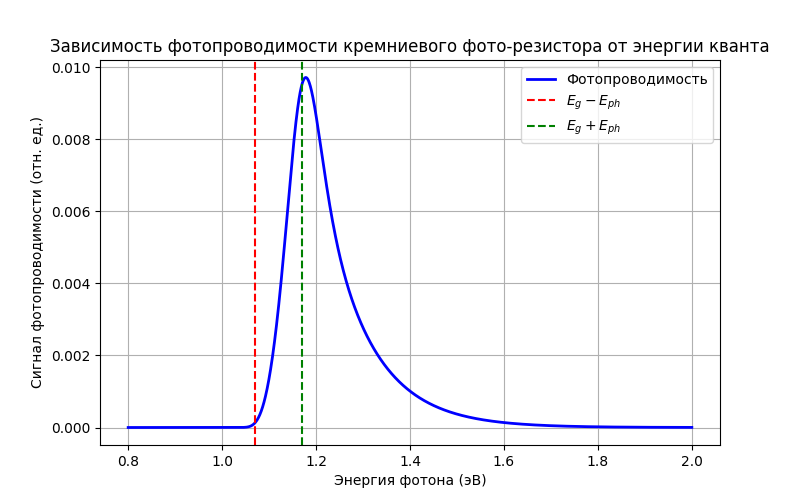
\includegraphics[scale=0.5]{img/10ans.png}
            \caption{}
    \end{figure}
    
\item Как зависит фотопроводимость $U/N$ при $kd \ll 1$ от $h \nu$ в прямозонных полупроводниках?
В прямозонных полупроводниках для энергий фотонов, близких к ширине запрещённой зоны \(E_g\), коэффициент поглощения имеет вид:
\[
\alpha(h\nu) = K_{d1}(h\nu - E_g)^n,
\]
где \(K_{d1}\) --- константа, зависящая от материала, а показатель степени \(n\) определяется характером оптического перехода.

\bigskip

Разрешённые переходы:

При разрешённых переходах оптический момент ненулевой, а плотность состояний приводит к зависимости
\[
\alpha(h\nu) \sim (h\nu - E_g)^{1/2}.
\]
При условии, что фотопроводимость пропорциональна количеству поглощённых фотонов, получаем:
\[
\frac{U}{N} \sim \alpha(h\nu) \sim (h\nu - E_g)^{1/2}.
\]

\bigskip

Запрещённые переходы:

При запрещённых переходах оптический момент равен нулю при прямом переходе, и переход возможен только с участием фононов или вследствие нарушения правил отбора, что приводит к дополнительному энергетическому множителю:
\[
\alpha(h\nu) \sim (h\nu - E_g)^{3/2}.
\]
Таким образом,
\[
\frac{U}{N} \sim (h\nu - E_g)^{3/2}.
\]

\bigskip

Подытожим, зависимость фотопроводимости от энергии фотона выглядит следующим образом:
\[
\frac{U}{N} \sim
\begin{cases}
(h\nu - E_g)^{1/2}, & \text{при разрешённых переходах}, \\
(h\nu - E_g)^{3/2}, & \text{при запрещённых переходах.}
\end{cases}
\]

Эта зависимость вытекает из учёта плотности состояний и правил отбора для оптических переходов в прямозонных полупроводниках

\item На Рис. 6 приведены результаты измерения сигнала  U фотопроводимости (ФП) образца CdSe  в зависимости от энергии $h \nu$ падающего на образец света. Этот ПП – прямозонный.
Оцените ширину запрещенной зоны CdSe.

\begin{figure}[!h]
        \centering
        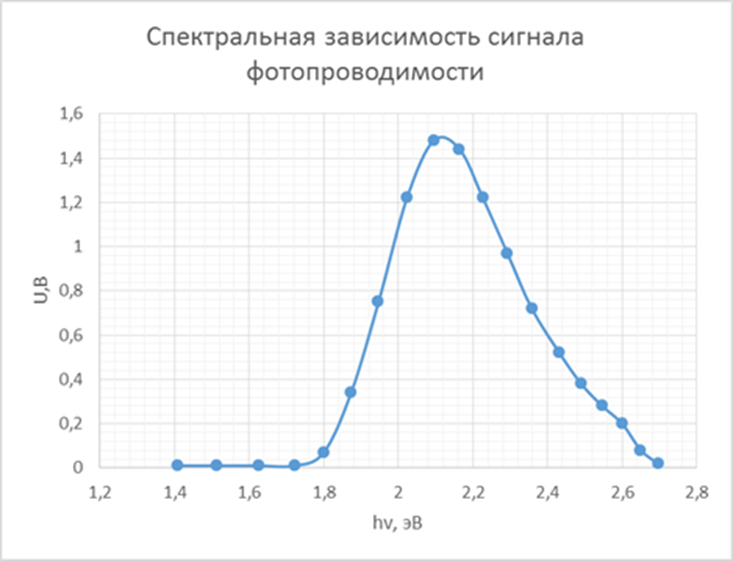
\includegraphics[scale=0.7]{img/12.png}
        \caption{}
\end{figure}

\itemРассчитать удельное сопротивление кремния, данные – в таблице в конце описания работы.

1. Определение концентрации носителей

Концентрация носителей определяется по формуле:
\[
n_i = \sqrt{N_c N_v}\, \exp\left(-\frac{E_g}{2 k_B T}\right),
\]
где:
\begin{itemize}
    \item \( N_c = 2.8\times10^{19}\,\text{см}^{-3} \) --- эффективная плотность состояний в зоне проводимости,
    \item \( N_v = 1.02\times10^{19}\,\text{см}^{-3} \) --- эффективная плотность состояний в валентной зоне,
    \item \( E_g = 1.11\,\text{эВ} \) --- ширина запрещённой зоны,
    \item \( k_B = 8.617\times10^{-5}\,\text{эВ/K} \) --- постоянная Больцмана,
    \item \( T = 300\,\text{K} \) --- абсолютная температура.
\end{itemize}

Подставляем данные:
\[
n_i = \sqrt{(2.8\times10^{19})(1.02\times10^{19})}\, \exp\left(-\frac{1.11}{2\cdot8.617\times10^{-5}\cdot300}\right).
\]

Сначала вычислим предфактор:
\[
\sqrt{N_c N_v} = \sqrt{2.8\times10^{19}\cdot1.02\times10^{19}} \approx \sqrt{2.856\times10^{38}} \approx 1.69\times10^{19}\,\text{см}^{-3}.
\]

Вычисляем показатель экспоненты:
\[
\frac{E_g}{2 k_B T} = \frac{1.11}{2\cdot8.617\times10^{-5}\cdot300} \approx \frac{1.11}{0.0517} \approx 21.45.
\]
Таким образом,
\[
n_i \approx 1.69\times10^{19}\,\text{см}^{-3}\cdot \exp(-21.45) \approx 1.69\times10^{19}\cdot 4.8\times10^{-10} \approx 8.1\times10^{9}\,\text{см}^{-3}.
\]

2. Расчёт проводимости и удельного сопротивления

Проводимость внутреннего полупроводника определяется по формуле:
\[
\sigma = q\, n_i\, (\mu_n + \mu_p),
\]
где:
\begin{itemize}
    \item \( q = 1.602\times10^{-19}\,\text{C} \) --- элементарный заряд,
    \item \( \mu_n \approx 1350\,\text{см}^2/(\text{В}\cdot\text{с}) \) --- подвижность электронов,
    \item \( \mu_p \approx 480\,\text{см}^2/(\text{В}\cdot\text{с}) \) --- подвижность дырок.
\end{itemize}

Суммарная подвижность равна:
\[
\mu_n + \mu_p \approx 1350 + 480 = 1830\,\text{см}^2/(\text{В}\cdot\text{с}).
\]

Подставляем значения:
\[
\sigma \approx 1.602\times10^{-19}\cdot 8.1\times10^{9}\cdot 1830 \approx 2.37\times10^{-6}\,\text{См/см}.
\]

Удельное сопротивление \(\rho\) находится по соотношению:
\[
\rho = \frac{1}{\sigma} \approx \frac{1}{2.37\times10^{-6}} \approx 4.21\times10^{5}\,\Omega\cdot\text{см}.
\]

Таким образом, удельное сопротивление кремния при \( T = 300\,\text{K} \) составляет:
\[
\boxed{\rho \approx 4.2\times10^{5}\,\Omega\cdot\text{см}}.
\]


\item По спектрам поглощения (см методичку) показать область прямых и непрямых переходов в Si и Ge


\end{enumerate}
\section{Ответы на вопросы к лабораторной работе №7}
\begin{enumerate}
    \item Дайте определение скорости поверхностной рекомбинации.

Скорость поверхностной рекомбинации  - это количество носителей заряда в 1 см$^{-3}$, рекомбинирующих на 1 см$^2$ поверхности в единицу времени. То есть:

$$s=\frac{S-S_0}{n-n_0}=\frac{1}{4}v(1-r),$$

где $S$ - скорость генерации электронов на единичной площадке, $v$ - средняя тепловая скорость, $r$ - средняя вероятность отражения носителя заряда от поверхности.
    
    \item Оцените диффузионную длину $L$, считая, что объемное время жизни в образце $Si$ составляет
 $\tau\approx 10^{-4}$ с. Проверьте, выполняется ли условие $KL>>1$ и $Kd>>1$ (толщина образца в направлении  освещения 0,55мм).\par
 Этот вопрос был в прошлой лабораторной работе, он решён.
    \item Поясните понятие «амбиполярная диффузия». Выведите формулу для коэффициента амбиполярной диффузии D.\par
    амбиполярная диффузия - совместное перемещение электронов и дырок вглубь образца под действием градиента концентраций. Электроны диффундируют быстрее, опережают дырки, и в образце возникает электрическое поле, которое тормозит электроны и ускоряет дырки. В результате электроны и дырки двигаются вместе с общим коэффициентом диффузии, который называется коэффициент амбиполярной диффузии.\par
    Вывод формулы: Для простоты ограничимся одномерным случаем и будем считать, что градиент концентрации и внешнее электрическое поле направлены вдоль оси х. Тогда уравнения непрерывности и уравнение для плотности токов должны быть записаны как для электронов, так и для дырок:
    \[
    \frac{\partial\Delta n}{\partial t}= \frac{1}{e}\frac{\partial j_n}{\partial x} - \frac{\Delta n}{\tau}
    \]
    \[
    \frac{\partial\Delta p}{\partial t}= \frac{1}{e}\frac{\partial j_p}{\partial x} - \frac{\Delta p}{\tau}
    \]
    \[
    j_n = en\mu_n E + eD_n\frac{d(\Delta n)}{dx}
    \]
      \[
    j_p = ep\mu_p E + eD_p\frac{d(\Delta p)}{dx}
    \]
    \par
    Для того чтобы определить $\mu_E$ и $D$, запишем уравнения непрерывности, подставив в них значения $j_n$ и $j_p$:
    \[
    \frac{\partial\Delta n}{\partial t}= D_n\frac{1}{e}\frac{\partial j_n}{\partial x} - \frac{\Delta n}{\tau}
    \]
    \[
    \frac{\partial\Delta p}{\partial t}=- \frac{1}{e}\frac{\partial j_p}{\partial x} - \frac{\Delta p}{\tau}
    \]
    Умножив полученные уравнения соответственно на $\sigma_p = ep\mu_p$ и $\sigma_n = en\mu_n$, сложим оба уравнения. В результате, учитывая что $\Delta n =\Delta p$и используя соотношение Эйнштейна, получаем:
    \[
    \frac{\partial\Delta n}{\partial t}= \frac{D_n \sigma_p +D_p \sigma_n}{\sigma_p + \sigma_n} \frac{\partial^2(\Delta n)}{\partial x^2} +\frac{\mu_n \sigma_p - \mu_p \sigma_n}{\sigma_p +\sigma_n}E\frac{\partial(\Delta n)}{\partial t} - \frac{\Delta n}{\tau}    \]
    Для стационарного случая, когда $\frac{\partial\Delta n}{\partial t} = 0$, уравнение можно записать в следующем виде:
    \begin{equation}
        \frac{D_n \sigma_p +D_p \sigma_n}{\sigma_p + \sigma_n} \frac{\partial^2(\Delta n)}{\partial x^2} +\frac{\mu_n \sigma_p - \mu_p \sigma_n}{\sigma_p +\sigma_n}E\frac{\partial(\Delta n)}{\partial t} - \frac{\Delta n}{\tau} = 0
    \end{equation}
    Учитывая, что при $n \approx n_0$ и $p \approx p_0$,  аэто справедливо когда $\Delta n <<n_0 $ и $\Delta p << p_0 $ и используя соотношение Эйнштейна для электронов и дырок $\frac{\mu_n}{D_n} = \frac{\mu_p}{D_p} = \frac{e}{kT}$, коэффициент амбиполярной диффузии можно записать в виде:
    \begin{equation}
        D = \frac{D_n \sigma_p + D_p \sigma_n}{\sigma_p + \sigma_n} = \frac{n_0+p_0}{\frac{n_0}{D_p}+ \frac{p_o}{D_n}} = \frac{kT}{e}\frac{n_0+p_0}{\frac{n_0}{\mu_p}+\frac{p_0}{\mu_n}}
    \end{equation}
    а амбиполярную дрейфовую подвижность в виде:
    \begin{equation}
        \mu_E = \frac{\mu_n \sigma_p - \mu_p \sigma_n}{\sigma_p +\sigma_n} = \frac{p_0-n_0}{\frac{n_0}{\mu_p} + \frac{p_0}{\mu_n}}     
    \end{equation}
    Если воспользоваться соотношением Эйнштейна, коэффициент амбиполярной диффузии $D $ можно представить в виде:
    \[
    D = \frac{kT}{e} \mu_D
    \]
    \item По значениям подвижности  $\mu$ (см. Приложение) определите коэффициент амбиполярной диффузии в собственном кремнии.\par
    \[kT = [T=300K] = 25.9 [\text{мэВ}]\]
    Как обсуждалось выше, формула для коэффициента амбиполярной диффузии записывается как:
    \[
    D = \frac{kT}{e} \mu_D
    \]
    Подвижности электронов и дырок в кремнии равны: 1500 и 600 $\text{см}^2/(\text{В} \cdot \text{с})$. Так как полупроводник собственный, то амбиполярная подвижность из формул равна:
    \[
    \mu_D = 2\frac{\mu_n \mu_p}{\mu_n + \mu_p} = 857  [\text{см}^2/(\text{В}\cdot \text{с)}]
    \]
    Тогда коэффициент $D$:
    \[
    D = \frac{kT}{e} \mu_D = \frac{25.9 \cdot 10^{-3} \cdot 1.6 \cdot 10^{-19}}{1.6\cdot10^{-19}} 857 = 22.1 [\text{см}^2/c]
    \]
    
\end{enumerate}
\section{Список литературы}
\begin{itemize}
    \item Определение ширины запренщенной зоны полупроводников по спектральной зависимости фотопроводимости: лабораторная работа №3., О.И. Смирнова. -- Москва: МФТИ, 2021. -- 16 с.
    \item \textbf{Физика полупроводников.,} К.В.Шалимова, М.: Энергоатомиздат, 1985. -- 392 с.
\end{itemize}







\end{document}

